\section{Waveforms} The observed waveforms of the simulation of the hardware module will be discussed in the this section.

As reported in \cref{sec:usage}, the module shall be reset at startup. On reset, it can observed that the \lstinline{dout_valid} signal is set to zero. The simulation, which starts by loading the key, is started after the \lstinline{rst} signal's posedge.

It can also be observed that each cycle an input is fed, and the corresponding output is available at the next clock cycle, as per specification.
\begin{figure}[!ht]
    \centering
    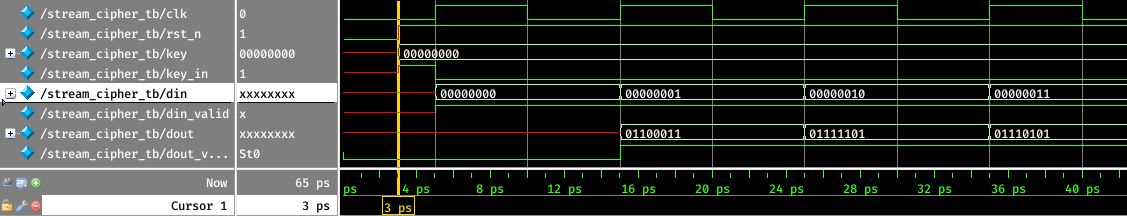
\includegraphics[width=1\textwidth]{startup_waveform}
    \caption{Startup waveform}
    \label{fig:startup_waveform}
\end{figure}

The following is the waveform for a key change. Note that in the cycle next to the key change there is no output, therefore \lstinline{dout_valid} will always be deasserted.
\begin{figure}[!ht]
    \centering
    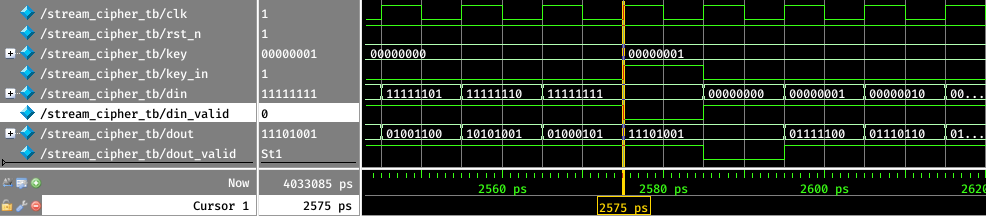
\includegraphics[width=1\textwidth]{key_change}
    \caption{Key change}
    \label{fig:key_change}
\end{figure}

The waveform of the \nth{2} test (see \cref{sec:tests}) has been reported here. It can be seen that, independently from the number of clock cycles the module waits, all signals follow the specification.
\begin{figure}[!ht]
    \centering
    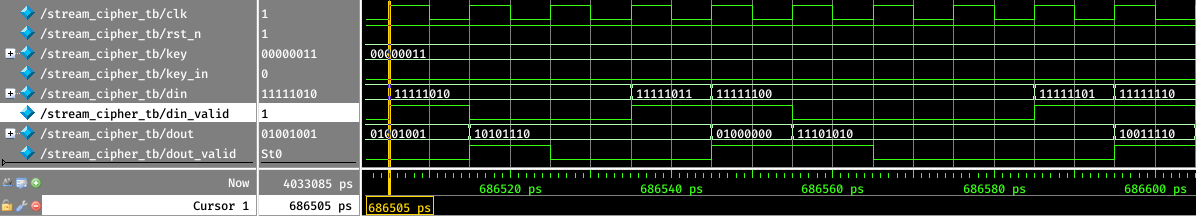
\includegraphics[width=1\textwidth]{random_waveform}
    \caption{Encryption waiting a random number of clock cycles}
    \label{fig:random_waveform}
\end{figure}

\clearpage
Finally, the waveform of the \nth{3} test (see \cref{sec:tests}) has been reported below.
\begin{figure}[!ht]
    \centering
    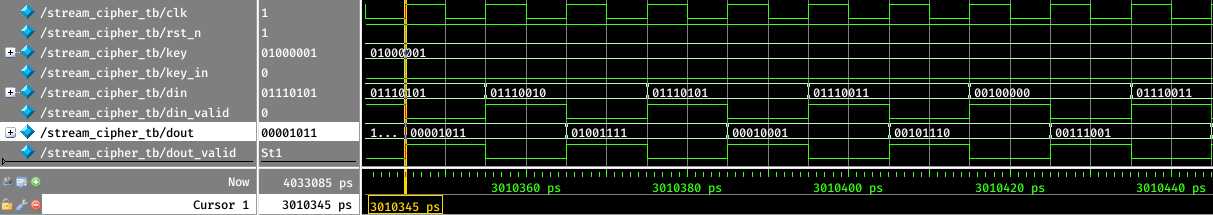
\includegraphics[width=1\textwidth]{file_encryption}
    \caption{File encryption/decryption waveform}
    \label{fig:file_encryption}
\end{figure}